\documentclass[conference]{IEEEtran}

\usepackage{newtxtext,newtxmath}
\usepackage{amsmath}
\usepackage{booktabs}
\usepackage{graphicx}
\usepackage{microtype}
\usepackage{multirow}
\usepackage{url}
\usepackage{xcolor}
\usepackage[hidelinks]{hyperref}
\usepackage{tikz}
\usetikzlibrary{arrows.meta,positioning,calc,fit}

\newcommand{\method}{\textsc{GaussProof}}
\newcommand{\clip}{\operatorname{clip}}
\newcommand{\E}{\mathbb{E}}
\newcommand{\R}{\mathbb{R}}
\newcommand{\Normal}{\mathcal{N}}

\title{\method: Repeated Gradient Fingerprints Survive High-Noise DP-SGD Trajectories}
%GaussProof: Auditing Repeated Gradient Fingerprints in High-Noise DP-SGD Trajectories

\author{Anonymous submission}

\begin{document}
\maketitle

\begin{abstract}
Differentially private stochastic gradient descent (DP-SGD) adds Gaussian noise to clipped minibatch gradients, and formal accounting composes privacy loss over training. Empirical privacy evaluations, however, often inspect a final model or a short observation window. We study a white-box setting in which an observer sees repeated noisy gradients and model states and knows the gradient fingerprint of a candidate record, but not its hidden batch participation. We introduce \method, a trajectory audit that updates the candidate fingerprint at each checkpoint and accumulates Gaussian likelihood evidence across releases. A controlled analysis shows that increasing noise reduces detection at fixed exposure, whereas repeated evidence can strengthen detection when participation is frequent. On exact evolving MNIST CNN trajectories with noise multiplier four and per-round participation $q=0.5$, holdout AUC rises from 0.609 at 16 releases to 0.819 at 128. At the ordinary-sampling proxy $q=0.004$, a 20-identity sensitivity experiment is at chance after 128 releases. A new paired 80-identity holdout compares the trajectory with LiRA and RMIA attacks on the final model: at $q=0.5$, AUC is 0.818 for the trajectory and 0.830 for LiRA when public-query model accuracy is 66\%; their difference is not statistically clear. At a lower-utility learning rate, the trajectory beats LiRA, showing that an apparent interface advantage depends on the endpoint baseline and training setting. A 30-identity gallery replication finds 13--15\% exact known-image retrieval from 32 candidates, versus 3.1\% at random; distribution mismatch produces class-level confounds. These experiments establish a participation- and interface-dependent audit, not a claim that more noise reduces privacy or that unknown images are reconstructed.
\end{abstract}


\section{Introduction}

Differential privacy (DP) is designed to remain valid against arbitrary post-processing and auxiliary information~\cite{dwork2006calibrating,dwork2014algorithmic}. DP-SGD applies this principle to iterative learning: it clips each per-record gradient, aggregates a minibatch, adds Gaussian noise, and composes the privacy loss of all updates~\cite{abadi2016deep}. The formal guarantee therefore already accounts for a powerful observer who combines every permitted release. In practice, however, empirical discussions of gradient leakage often present one update, one reconstruction, or one final model. A large noise multiplier can make those isolated observations look harmless even when the system exposes a long sequence of correlated, data-dependent updates.

This paper asks a concrete safety question: \emph{can a weak record-specific gradient signal, hidden by high noise in a short window, become useful when the same observer follows an entire DP-SGD trajectory?} The question matters for federated learning servers, distributed training infrastructure, debugging and telemetry systems, and APIs that reveal intermediate checkpoints or optimizer updates. These interfaces can be white-box even when the eventual model release is black-box. Prior DP audits have shown that observing all model updates is a meaningful and formally permitted threat model~\cite{nasr2023tight}; our focus is the mechanism by which a natural record's changing gradient fingerprint persists across those updates.

We call the resulting audit \method. For a specified candidate record, the observer recomputes its clipped per-record gradient at every public checkpoint, subtracts a public estimate of the minibatch background, evaluates a Gaussian shift likelihood against the released update, and adds evidence through time. The detector does not see the private batch, the sampled Gaussian noise, or the candidate's hidden inclusion schedule. Its computation is a matched filter over a time-varying fingerprint bank. This simple construction is important: in the high-noise regime, our learned sequence models and diffusion denoisers do not outperform the analytic likelihood score.

Figure~\ref{fig:framework} summarizes the audit. The method makes a stronger access assumption than final-model membership inference: the observer has model states, gradient releases, and a candidate record. We therefore report it as a white-box trajectory audit rather than as a universal attack on deployed DP-SGD. The access is realistic only where intermediate updates are exposed or where an internal participant is adversarial.

\begin{figure*}[t]
  \centering
  \resizebox{\textwidth}{!}{%
    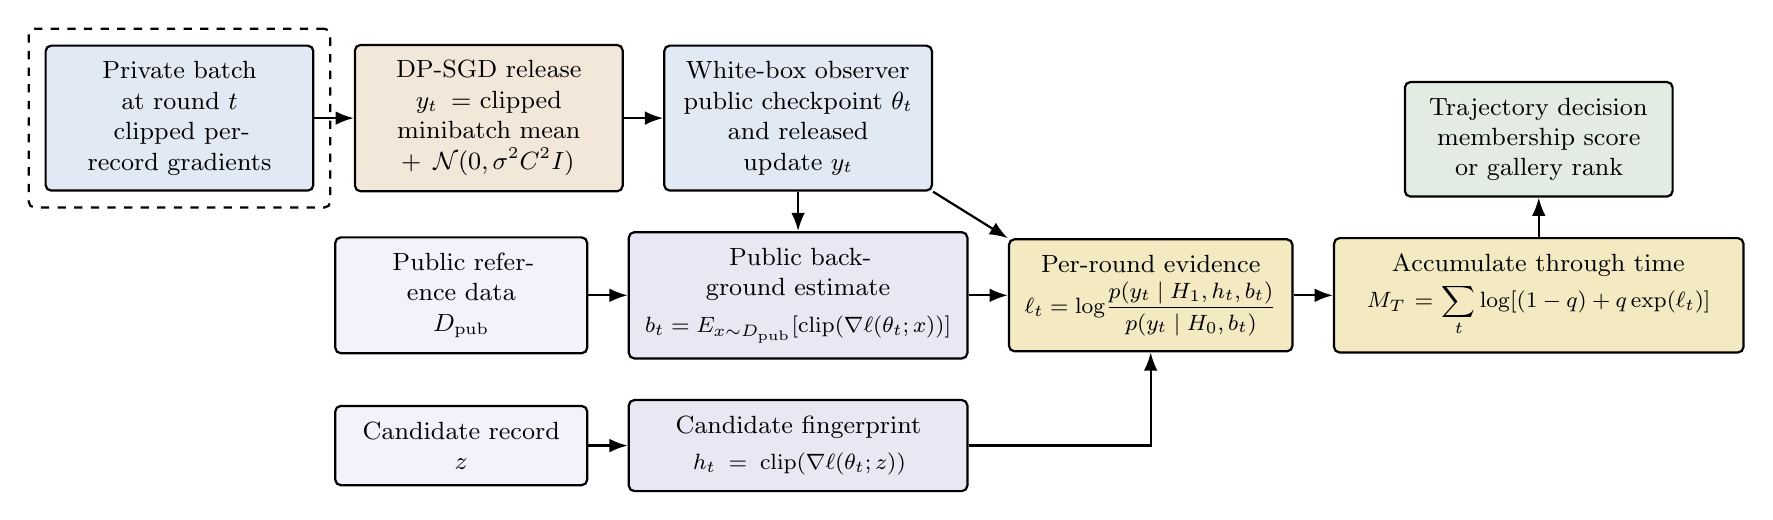
\begin{tikzpicture}[
  >=Latex,
  font=\small,
  box/.style={draw, rounded corners=2pt, thick, align=center, minimum height=11mm, text width=30mm, inner sep=2mm},
  mathbox/.style={draw, rounded corners=2pt, thick, align=center, minimum height=11mm, text width=39mm, inner sep=2mm},
  scorebox/.style={draw, rounded corners=2pt, thick, align=center, minimum height=12mm, text width=32mm, inner sep=2mm},
  accumbox/.style={draw, rounded corners=2pt, thick, align=center, minimum height=12mm, text width=48mm, inner sep=2mm},
  inputbox/.style={draw, rounded corners=2pt, thick, align=center, minimum height=9mm, text width=28mm, inner sep=2mm},
  flow/.style={->, thick},
  hidden/.style={draw, dashed, rounded corners=2pt, thick, inner sep=2mm}
]
  \definecolor{boxblue}{RGB}{225,233,244}
  \definecolor{boxbeige}{RGB}{243,231,217}
  \definecolor{boxgreen}{RGB}{226,236,227}
  \definecolor{boxyellow}{RGB}{244,234,194}
  \definecolor{boxlav}{RGB}{234,231,245}

  %\node[font=\bfseries\Large, anchor=west] (title) at (0,4.25) {\textsc{GaussProof} audit};

  % Top row: mechanism and observation.
  \node[box, fill=boxblue, anchor=west] (private) at (0,2.05)
    {Private batch at round $t$\\clipped per-record gradients};
  \node[box, fill=boxbeige, right=5mm of private] (release)
    {DP-SGD release\\$y_t=$ clipped minibatch mean\\$+\;\Normal(0,\sigma^2 C^2 I)$};
  \node[box, fill=boxblue, right=5mm of release] (observer)
    {White-box observer\\public checkpoint $\theta_t$\\and released update $y_t$};

  % Candidate-conditioned quantities are stacked so their connections to the
  % likelihood box remain visually separate.
  \node[mathbox, fill=boxlav, below=5mm of observer] (background)
    {Public background estimate\\[0.8mm]
     {\footnotesize $b_t=\E_{x\sim D_{\mathrm{pub}}}\!\left[\clip(\nabla\ell(\theta_t;x))\right]$}};
  \node[mathbox, fill=boxlav, below=5mm of background] (fingerprint)
    {Candidate fingerprint\\[0.8mm]
     {\footnotesize $h_t=\clip(\nabla\ell(\theta_t;z))$}};

  \node[scorebox, fill=boxyellow, right=5mm of background] (roundscore)
    {Per-round evidence\\[0.8mm]
     {\footnotesize $\displaystyle \ell_t=\log\!\frac{p(y_t\mid H_1,h_t,b_t)}{p(y_t\mid H_0,b_t)}$}};
  \node[accumbox, fill=boxyellow, right=5mm of roundscore] (accum)
    {Accumulate through time\\[0.8mm]
     {\footnotesize $\displaystyle M_T=\sum_t\log\!\left[(1-q)+q\exp(\ell_t)\right]$}};
  \node[box, fill=boxgreen, above=5mm of accum] (decision)
    {Trajectory decision\\membership score or gallery rank};

  % Public and candidate inputs.
  \node[inputbox, fill=boxlav!55, left=5mm of background] (pubdata)
    {Public reference data\\$D_{\mathrm{pub}}$};
  \node[inputbox, fill=boxlav!55, left=5mm of fingerprint] (candidate)
    {Candidate record\\$z$};

  % Main DP-SGD trajectory.
  \draw[flow] (private.east) -- (release.west);
  \draw[flow] (release.east) -- (observer.west);

  % Public and candidate-conditioned quantities.
  \draw[flow] (observer.south) -- (background.north);
  \draw[flow] (observer.south east) -- (roundscore.north west);
  \draw[flow] (pubdata.east) -- (background.west);
  \draw[flow] (candidate.east) -- (fingerprint.west);

  % Three distinct inputs to the per-round likelihood.  Each arrow terminates
  % on a box boundary and no connector crosses another box.
  \draw[flow] (background.east) -- (roundscore.west);
  \draw[flow] (fingerprint.east) -| ([xshift=0mm]roundscore.south);

  % Temporal accumulation and final decision.
  \draw[flow] (roundscore.east) -- (accum.west);
  \draw[flow] (accum.north) -- (decision.south);

  % Hidden information: keep this annotation compact and local to the private
  % side so it cannot overlap the likelihood connectors.
  \node[hidden, fit=(private)] (hiddenbox) {};
  %\node[anchor=north west, font=\small, align=left, text width=60mm]
  %  at ($(private.south west)+(0,-0.95)$)
  %  {Hidden from the observer: private batch contents, hidden inclusion schedule $I_t$, and sampled Gaussian noise.};
\end{tikzpicture}

  }
  \caption{\method~follows an evolving DP-SGD trajectory. At round $t$, the observer uses the public checkpoint $\theta_t$, released update $y_t$, public reference data $D_{\mathrm{pub}}$, and candidate record $z$ to form a public background estimate $b_t$, a candidate-specific clipped gradient fingerprint $h_t$, a per-round likelihood ratio $\ell_t$, and an accumulated trajectory score $M_T$. The observer never receives the private batch, hidden inclusion schedule, or sampled Gaussian noise.}
  \label{fig:framework}
\end{figure*}

Our evaluation is deliberately staged. First, a fixed-access Gaussian study holds fingerprints and hypotheses constant and confirms that more noise reduces optimal detection at fixed exposure. Second, exact evolving CNN experiments separate calibration and holdout canary identities and compare the last released update with 16-release trajectories at three noise multipliers. Third, we fix the hardest tested noise multiplier, $\sigma=4$, and extend the same paired trajectories from 16 to 128 releases. Fourth, we vary $q$ from 0.5 to 0.004 on 20 unseen identities and compare trajectory access with a true final-checkpoint attack. We then expand to 80 independent evaluation identities, stronger final-model LiRA/RMIA attacks, and an exploratory higher-utility training condition. Finally, we translate detection evidence into exact record recovery from an auxiliary gallery and vary the private class distribution.

The main findings are:
\begin{itemize}
  \item At fixed 16-round exposure, increasing $\sigma$ from 0.25 to 4 lowers unseen-canary AUC from 0.929 to 0.609. This is consistent with the DP mechanism and rules out the claim that noise intrinsically ``backfires.''
  \item At fixed $\sigma=4$, extending the same trajectories from 16 to 128 releases raises AUC from 0.609 to 0.819. The paired gain is 0.211 with a 95\% identity-clustered bootstrap interval $[0.144,0.272]$.
  \item The effect attenuates sharply with participation. At 128 releases, the $q$-aware trajectory AUC is 0.805 at $q=0.5$, 0.571 at $q=0.1$, and 0.503 at $q=0.004$. A final-checkpoint loss attack reaches 0.730, 0.549, and 0.498, respectively; the measured trajectory advantage is not statistically clear in this pilot.
  \item In the 80-identity replication at $q=0.5,T=128$, trajectory AUC is 0.810 versus final-model LiRA's 0.693 when model accuracy is only 24\%. At a calibration-selected, higher-utility learning rate with 66\% accuracy, the trajectory reaches 0.818 but LiRA reaches 0.830; the paired difference interval $[-0.043,0.020]$ includes zero. A simple raw trajectory alignment and a LiRA--trajectory fusion also fail to show a clear gain over LiRA.
  \item A BiLSTM and conditional diffusion detector do not improve high-noise AUC: they reach 0.610 and 0.566, respectively, versus 0.609 for the analytic score. In this pilot, the privacy signal is better exposed by accumulation than by a more expressive learned denoiser.
  \item In a 30-identity replication with a 32-image gallery, the correct held-out MNIST record is ranked first in 13--15\% of trials across four matched-background distributions, versus 3.1\% at random. With the target removed, only limited semantic leakage remains; this is candidate re-identification, not unknown-image synthesis.
  \item A mismatched public background can expose the dominant class while failing to distinguish individuals within that class. We introduce a same-class rank control to identify this failure mode.
\end{itemize}

These results do not contradict DP. Our conservative replace-one accounting without sampling amplification gives $\epsilon\leq 11.60$ at 16 rounds and $\epsilon\leq 43.14$ at 128 rounds for $\delta=10^{-5}$, so the evaluated long-trajectory setting is a weak-privacy regime. The security lesson is that a large per-release noise multiplier is not a stand-alone privacy statement. Release count, sampling, the observer's interface, and composition determine the guarantee and must also determine the audit.

\section{Background and Related Work}

\subsection{DP-SGD and Composition}

Two datasets are adjacent if one can be obtained from the other by replacing a single record. A randomized mechanism $M$ is $(\epsilon,\delta)$-DP if, for all adjacent $D,D'$ and measurable output events $O$,
\begin{equation}
\Pr[M(D)\in O]\leq e^\epsilon\Pr[M(D')\in O]+\delta.
\end{equation}
The guarantee bounds all inferences from the mechanism's output, including those made with auxiliary data. Smaller $\epsilon$ and $\delta$ give stronger protection, but the reported parameters are only meaningful when the mechanism, adjacency, sampling, and number of compositions are specified.

At model state $\theta_t$, DP-SGD computes per-record gradients $g_t(z)=\nabla_\theta\ell(\theta_t;z)$ and clips them to
\begin{equation}
h_t(z)=\clip_C(g_t(z))=g_t(z)\min\left(1,\frac{C}{\lVert g_t(z)\rVert_2}\right).
\end{equation}
For a fixed-size batch $S_t$ of size $B$, the released averaged gradient is
\begin{equation}
y_t=\frac{1}{B}\left(\sum_{z\in S_t}h_t(z)+n_t\right),
\qquad n_t\sim\Normal(0,\sigma^2 C^2 I),
\label{eq:dpsgd}
\end{equation}
followed by $\theta_{t+1}=\theta_t-\eta y_t$. Rényi DP, zero-concentrated DP (zCDP), and Gaussian DP provide convenient composition views~\cite{mironov2017renyi,bun2016concentrated,dong2022gaussian}. For a replace-one sensitivity upper bound $2C$ on the gradient sum, a conservative per-round zCDP value is $\rho=2/\sigma^2$. Across $T$ releases, $\rho_T=2T/\sigma^2$, which converts to
\begin{equation}
\epsilon\leq \rho_T+2\sqrt{\rho_T\log(1/\delta)}.
\label{eq:zcdp}
\end{equation}
We report this loose no-amplification bound to make exposure explicit. It is not an estimate of empirical leakage and should not replace an accountant matched to the actual sampler. Recent work demonstrates that sampling details can create a substantial gap between intended and implemented DP-SGD accounting \cite{chua2024private}.

\subsection{Membership Inference and DP Auditing}

Membership inference asks whether a record contributed to training. Output confidence and shadow models are classic black-box approaches \cite{shokri2017membership}; likelihood-ratio attacks make the hypothesis test explicit and improve power~\cite{carlini2022membership,zarifzadeh2024lowcost}. DP auditing instead uses attacks to estimate or falsify an implementation's privacy behavior. Poisoning-based and influence-based audits improve statistical power~\cite{jagielski2020auditing,lu2022general}, while update-level access can produce tight audits on natural data with few training runs \cite{nasr2023tight}. Randomized canaries and one-run methods further reduce the cost of obtaining valid empirical lower bounds \cite{pillutla2023randomization,steinke2023one}. Black-box audits can also become nearly tight under carefully designed initializations~\cite{annamalai2024blackbox}.

Prior work also studies privacy when multiple training states are available. Jagielski et al.~\cite{jagielski2023updates} combine membership evidence across updated models and show that access to model updates can strengthen membership inference. Cherubin et al.~\cite{cherubin2024closed} model DP-SGD as an information-theoretic channel whose outputs include intermediate model parameters and derive closed-form record-level inference bounds. Separately, privacy-amplification-by-iteration analyses show that concealing intermediate states can, under additional assumptions, yield tighter guarantees than composition bounds that remain valid when those states are exposed \cite{feldman2018iteration,ye2022hidden}. These results motivate treating the release interface itself as part of the privacy threat model.

Our goal differs from estimating a tight empirical $\epsilon$ or deriving a new composition law. We construct a candidate-conditioned, time-varying likelihood on exact evolving white-box DP-SGD trajectories with hidden per-round participation, test transfer to unseen natural candidates, and use identity-aware gallery controls to distinguish record linkage from class- or distribution-level leakage. Consequently, our results quantify attack discrimination under the stated distribution rather than certify a general privacy lower bound.

\subsection{Gradient Reconstruction and Learned Priors}

Unprotected gradients can reveal training inputs. Deep Leakage from Gradients optimizes dummy records to match an observed gradient~\cite{zhu2019deep}, and later work improves fidelity with stronger image priors and objectives \cite{geiping2020inverting}. Under structural conditions, training data can even be identifiable from a gradient and recovered by efficient tensor methods \cite{wang2023reconstructing}. These attacks commonly target one or a small number of relatively clean updates. Additive noise and larger batches make pixel reconstruction substantially harder.

Learned denoisers can exploit structure in a protected domain. RAoPT uses an LSTM trained on clean and protected location trajectories to partially undo trajectory publication noise~\cite{buchholz2022raopt}. Diffusion models learn a denoising process~\cite{ho2020denoising}; recent gradient-guided conditional diffusion work applies such priors to noise-perturbed federated gradients \cite{meng2026enhanced}. These results motivate our learned controls. They do not imply that a diffusion model can remove DP noise without auxiliary signal: the DP post-processing guarantee still applies, and a Bayes estimator can only exploit a prior plus information present in the release.

\section{Threat Model and Evaluation Scope}

\subsection{System and Observer}

We consider a training service that exposes the sequence $\{(\theta_t,y_t)\}_{t=1}^{T}$, where $y_t$ is the actual noisy gradient used to update the model. The observer knows the architecture, loss, clipping threshold $C$, noise multiplier $\sigma$, batch size $B$, learning rate, and sampling protocol. This is an internal or federated-server threat model, not a final-model API. For vanilla SGD with known learning rate, exposing every consecutive model state already reveals the corresponding update through $y_t=(\theta_t-\theta_{t+1})/\eta$; a separate gradient-logging channel is therefore unnecessary when all consecutive checkpoints are visible. The observer also possesses a candidate record $z_c=(x_c,y_c)$ or a finite gallery of candidate records. Such auxiliary access models an auditor-inserted canary or an attacker with a suspected record list.

The observer may train on disjoint public data and use it to estimate the mean gradient of an ordinary batch. It cannot read the private population, batch membership, candidate inclusion indicator $a_t$, or sampled noise $n_t$. It cannot change the training data or gradients. We therefore study a passive white-box observer with auxiliary fingerprints.

The candidate can be either absent at all rounds ($H_0$) or eligible for independent inclusion with probability $q$ at each round ($H_1$). This participation schedule is deliberately controlled by the experiment and need not match the inclusion probability of an ordinary record under uniform minibatch sampling. The evolving model makes the candidate fingerprint time-dependent. The primary membership task ranks a trajectory under $H_1$ versus $H_0$. The gallery task ranks multiple known candidates. In both cases, the private observation is unchanged; candidate fingerprints are recomputed from public states.

\subsection{Scope of the Audit}

An exact gallery match establishes record linkage: the released trajectory identifies which known record participated. It is relevant when an attacker already has a finite list of suspected records. It is not free-form image reconstruction. We reserve the latter term for recovering target-specific pixel information when the target is absent from every attack prior or gallery.

Our evaluation first tests whether trajectory accumulation transfers to unseen natural canaries and how detection changes with $\sigma$ at fixed exposure. We then examine whether weak evidence strengthens along longer prefixes of the same high-noise DP-SGD trajectories and whether learned BiLSTM or diffusion sequence models improve on the analytic detector. Finally, we test whether the accumulated evidence supports closed-gallery record linkage across training distributions and use distribution-shift controls to identify cases where class-level leakage can masquerade as identity recovery.

\section{GAUSSPROOF}

\subsection{A Time-Varying Gradient Fingerprint}

At round $t$, the candidate fingerprint is $h_t=h_t(z_c)$. Let $b_t$ denote the expected clipped gradient of an ordinary population record under the observer's public background model. If candidate inclusion replaces one ordinary batch record, the mean shift in the averaged release is
\begin{equation}
s_t=\frac{h_t-b_t}{B}.
\label{eq:shift}
\end{equation}
The subtraction matters. A raw alignment $\langle h_t,y_t\rangle$ can respond to a common class or optimization direction. The residual $h_t-b_t$ asks what the candidate contributes beyond a typical replacement.

Approximating minibatch variation by its public mean and retaining the exact DP-noise variance gives
\begin{align}
H_0 &: y_t\sim\Normal(b_t,vI),\\
H_{1,t} &: y_t\sim\Normal(b_t+s_t,vI),
\qquad v=(\sigma C/B)^2.
\end{align}
The one-round Gaussian log-likelihood ratio (LLR) is
\begin{equation}
\ell_t=\frac{\langle s_t,y_t-b_t\rangle}{v}
-\frac{\lVert s_t\rVert_2^2}{2v}.
\label{eq:llr}
\end{equation}
The first term is a matched filter. The second penalizes candidates whose large fingerprint norm would otherwise dominate gallery ranking.

\subsection{Hidden Participation and Trajectory Evidence}

When the candidate participates with probability $q$, the round distribution under $H_1$ is a mixture of absent and present components. The exact mixture-to-null LLR under the approximation is
\begin{equation}
m_t=\log\left[(1-q)+q\exp(\ell_t)\right].
\label{eq:mixture}
\end{equation}
Assuming conditionally independent DP noise across rounds, the $q$-aware trajectory score is
\begin{equation}
M_T=\sum_{t=1}^{T}m_t.
\label{eq:trajectory}
\end{equation}
We refer to the overall candidate-conditioned trajectory audit as \method. Its $q$-aware likelihood score is $M_T$; we additionally report $L_T=\sum_t\ell_t$ as a simpler matched-score control. The two scores are similar empirically at $q=0.5$. For a gallery $\{z_j\}_{j=1}^K$, the observer recomputes every $h_{j,t}$ and returns $\arg\max_j M_T(z_j)$. The work is $O(TKd)$ for $d$ observed gradient coordinates and requires only streaming state $O(K)$ once each checkpoint's fingerprints are computed.

The model state itself depends on earlier private batches and noise. We do not freeze or replay checkpoints in the main trajectory experiments: fingerprints, backgrounds, releases, and updates are computed at the same evolving $\theta_t$. This preserves the temporal coupling that a real observer faces.

\subsection{Signal Accumulation Across High-Noise Releases}

Consider a fixed concatenated signal $H=(s_1,\ldots,s_T)$ and whitened noise variance $v$. The normalized matched statistic has
\begin{equation}
Z\sim\Normal(0,1)\quad\text{under }H_0,
\qquad
Z\sim\Normal(\mu,1)\quad\text{under }H_1,
\end{equation}
where
\begin{equation}
\mu^2=\sum_{t=1}^{T}\frac{\lVert s_t\rVert_2^2}{v}.
\label{eq:mu}
\end{equation}
For approximately stationary fingerprint energy, $\mu=\Theta(\sqrt{T}/\sigma)$. At false-positive rate $\alpha$, the optimal Gaussian power is
\begin{equation}
\operatorname{TPR}=\Phi\left(\mu-\Phi^{-1}(1-\alpha)\right).
\label{eq:power}
\end{equation}
Equation~\ref{eq:power} resolves the apparent paradox. Holding $T$ fixed, increasing $\sigma$ lowers $\mu$ and detection power monotonically. Holding $\sigma$ fixed, adding independent releases with nonzero fingerprint energy increases $\mu$. The same dependence appears in privacy composition: exposure increases with $T/\sigma^2$. There is no reversal of DP's privacy ordering. This accumulation viewpoint is also consistent with prior record-level analyses that treat intermediate DP-SGD states as outputs of an information-theoretic channel~\cite{cherubin2024closed}.

Hidden participation adds a second attenuation factor. In the fixed Gaussian
channel above, let $P_{0,t}=\Normal(0,vI)$ and
$P_{1,t}=(1-q)P_{0,t}+q\Normal(s_t,vI)$, with
$\kappa_t=\lVert s_t\rVert_2^2/v$. Direct integration of the Gaussian
likelihood ratio gives
\begin{equation}
\chi^2(P_{1,t}\Vert P_{0,t})=q^2\bigl(e^{\kappa_t}-1\bigr).
\label{eq:participation-chi2}
\end{equation}
For independent rounds, $1+\chi^2(P_1\Vert P_0)$ is the product of
$1+q^2(e^{\kappa_t}-1)$ over $t$. Consequently, when every $\kappa_t$ is
small, the distinguishability scale is approximately
$q\sqrt{\sum_t\kappa_t}$, or $q\sqrt{T}/\sigma$ for comparable
fingerprint energy. This is a diagnostic calculation for the fixed-background
Gaussian channel, not a privacy accountant or a bound asserted for adaptive
CNN training. It explains why large per-release noise and short exposure can
mask an infrequently participating record even when a high-$q$ canary remains
detectable over a long trajectory.

This calculation is a Gaussian hypothesis-testing specialization, not a new DP theorem or composition result. Real trajectories violate its fixed-background and conditional-independence approximations through minibatch variation and model evolution. Our exact training experiments test whether the operational candidate-conditioned detector retains the accumulation effect under those deviations.

\subsection{Learned Sequence Baselines}

We compare the analytic score with two learned models using the same available information. Seven dimensionless features are formed per round: LLR, normalized matched projection, fingerprint signal-to-noise ratio, observation RMS, cosine alignment, normalized round index, and $\log\sigma$. A bidirectional LSTM embeds the sequence and pools its mean and maximum hidden states for membership classification.

The diffusion control treats the hidden inclusion indicators $a_{1:T}\in\{0,1\}^T$ as the target sequence. A two-layer temporal Transformer is trained with a standard diffusion velocity objective, conditioned on the same seven features. DDIM sampling estimates the posterior inclusion schedule; mean reconstructed inclusion is used as the membership score. Identity cross-fitting prevents the evaluated canary from appearing in learned-model training. These models test whether nonlinear temporal structure helps; they do not receive clean gradients or the true inclusion schedule at inference.

\section{Experimental Setup}

\subsection{Dataset, Model, and Splits}

We use MNIST~\cite{lecun1998gradient} because exact per-record gradients for every parameter can be recomputed over many evolving trajectories on CPU. The model has two convolutional layers with 4 and 8 channels, $3\times3$ kernels, tanh activations and average pooling, followed by a 32-unit tanh layer and a 10-class head. Every attack gradient covers all model parameters.

One random permutation creates disjoint roles: 3,000 public pretraining records, 64 public background records, four calibration canaries, four holdout canaries, a 2,000-record private population, and 1,000 held-out records. The CNN is publicly pretrained for 100 nonprivate steps with batch size 64 and learning rate 0.1. The audit then starts from the identical public checkpoint for every paired condition. The participation-rate study selects the first two records of each digit from the persisted held-out role, giving 20 fixed identities; none is used in public pretraining, background estimation, or the private population. The gallery experiment draws a separate stratified 32-image gallery from the same held-out role; its first ten records, one per digit, act as the possible private contributors in the pilot, while a replication evaluates three records per digit (30 identities) with the same 32-image gallery.

Table~\ref{tab:setup} gives the audited DP-SGD configuration. The primary canaries are ordinary held-out MNIST records drawn from the same data distribution and subjected to the same clipping rule as population records. Their participation schedule is deliberately controlled: each positive trajectory includes its canary independently with probability $q$, whereas each negative trajectory excludes it. The primary study uses $q=0.5$; the sensitivity study adds $q\in\{0.1,0.02,0.004\}$, where 0.004 is approximately $B/N=8/2000$ under uniform fixed-size minibatch sampling. Other batch records are sampled without replacement from the private population. The release in Eq.~\ref{eq:dpsgd} is exactly the gradient used for the model update. Separate random generators control inclusion, batch sampling, and Gaussian noise. Shared seeds make every lower-$q$ inclusion schedule a subset of its paired higher-$q$ schedule.

\begin{table}[t]
\caption{Primary exact-trajectory configuration.}
\label{tab:setup}
\centering
\begin{tabular}{lc}
\toprule
Parameter & Value \\
\midrule
Dataset / model & MNIST / small CNN \\
Clipping norm $C$ & 1.0 \\
Batch size $B$ & 8 \\
Learning rate $\eta$ & 0.05 \\
Noise multipliers $\sigma$ & 0.25, 1, 4 \\
Canary inclusion $q$ & 0.5 \\
Sensitivity $q$ & 0.5, 0.1, 0.02, 0.004 \\
Short trajectory & 16 releases \\
Long prefixes at $\sigma=4$ & 16, 32, 64, 128 \\
Sequences per identity/hypothesis & 12 \\
Calibration / holdout identities & 4 / 4 \\
Sensitivity identities / repetitions & 20 / 3 \\
Privacy $\delta$ & $10^{-5}$ \\
\bottomrule
\end{tabular}
\end{table}

\subsection{Evaluation Protocol}

\emph{Fixed-access noise sweep.} Before dynamic training, we evaluate 90 real clipped gradient templates from three public CNN seeds and two checkpoints. Templates, labels, hypotheses, and 16 releases are fixed across nine noise levels. For each template and hypothesis, 20,000 paired Monte Carlo observations are evaluated through the exact projected sufficient statistic. This experiment checks the implementation against Eq.~\ref{eq:power} and establishes the fixed-exposure monotonic control.

\emph{Unseen-canary holdout.} For each $\sigma\in\{0.25,1,4\}$, the detector is calibrated on four canary identities and evaluated on four disjoint identities. Each identity has 12 positive and 12 negative 16-round trajectories, giving 48 positives and 48 negatives per holdout condition. Thresholds for 1\% and 5\% FPR are selected on calibration identities only.

\emph{Long high-noise trajectories.} At $\sigma=4$, we extend the exact same paired holdout sequences to 128 rounds and score nested prefixes of 16, 32, 64, and 128 releases. No prefix is simulated independently, which avoids confounding the comparison with independently sampled easier or harder trajectories. Longer prefixes nevertheless contain additional DP-SGD steps and therefore additional privacy expenditure; this experiment does not hold the overall privacy budget fixed.

\emph{Participation sensitivity and endpoint.} At $\sigma=4$, we run $q\in\{0.5,0.1,0.02,0.004\}$ on 20 stratified unseen identities with three paired positive and negative sequences per identity. We score the same prefixes as above. The trajectory detector uses the correct $q$ in Eq.~\ref{eq:mixture}. Its endpoint comparator is the negative cross-entropy of the known candidate under the model after step $T$; it receives only that final checkpoint and candidate, not the last update or any intermediate state. This produces 480 exact trajectories. The inclusion RNG is separate, and shared seeds make lower-$q$ schedules nested within higher-$q$ schedules.

\emph{Stronger endpoint replication.} We select 100 stratified identities from the held-out split: 20 (two per digit) for attack calibration, and 80 previously unevaluated identities (eight per digit) for final comparison. Each identity has one paired positive and negative trajectory at $q\in\{0.5,0.1\}$; the 64- and 128-update scores use prefixes of the same run. Thirty-two OUT reference models are trained with the same DP-SGD mechanism on a separate 2,000-record public MNIST pool. A further disjoint set of 128 public records provides RMIA's population comparison. We compute offline LiRA with a Gaussian OUT-logit score or one-sided standardized OUT logit, and offline RMIA~\cite{carlini2022membership,zarifzadeh2024lowcost} with $a\in\{0,0.5,1\}$ and $\gamma\in\{1,1.05\}$. The 20 calibration identities select variants; no holdout labels fit the attacks. Endpoint attacks see only the final model, candidate, and public reference predictions. Full-trajectory scores see all released updates and checkpoints. We also report raw candidate-gradient alignment as a same-access control; it is not a full reproduction of RERO's informed reconstruction algorithm. A 20-identity calibration-only screen over learning rates $\{0.005,0.01,0.02,0.05\}$ selected $0.005$ to test whether the endpoint comparison persists when model utility improves. This follow-up rate is exploratory, while the 80 evaluation identities remain untouched by selection.

\emph{Learned comparison.} Fourfold identity cross-fitting trains the BiLSTM and diffusion detector without the evaluated identity. Model selection uses calibration identities. Analytic and learned scores receive identical sequence features and are evaluated on the same 16-round holdout trajectories.

\emph{Gallery and distribution shift.} The pilot runs two trajectories for each of ten true gallery identities. We replicate with 30 identities, three per digit, and two trajectories each under four private label distributions: balanced, long-tail with probability proportional to $1/(k+1)$ for digit $k$, canary class rare with probability 0.05, and canary class dominant with probability 0.70. The replication therefore contains 240 exact trajectories. Paired noise seeds are shared across distributions. The primary background model matches the private class distribution; a robustness model remains balanced. All gallery candidates are available under both hypotheses.

\subsection{Metrics and Uncertainty}

Membership detection uses tie-aware ROC AUC. Low-FPR results report the realized holdout TPR and FPR at calibration-selected thresholds. For both trajectory studies, 2,000 paired cluster-bootstrap repetitions resample canary identities and positive/negative sequence indices together. The original long-trajectory study has four identities; the participation study increases this to 20 while reducing repetitions per identity from 12 to three.

The stronger endpoint replication uses 1,000 paired identity-bootstrap samples of its 80 holdout identities. Its 20 negative calibration identities resolve a nominal 5\% FPR threshold only coarsely; we report achieved holdout FPR beside TPR and make no calibrated 1\% FPR claim. Public-query classification accuracy is measured on the disjoint 128-record RMIA population to expose low-utility comparisons.

Gallery evaluation reports exact top-1, top-5, mean reciprocal rank, predicted digit agreement, and same-class top-1. Same-class rank restricts candidates to the true digit, separating identity evidence from class recognition. An open-gallery control removes the true image before selecting the best alternative, then reports digit agreement and pixel MSE. With 32 candidates, random top-1 is 3.125\%, top-5 is 15.625\%, and expected random MRR is 0.127. An oracle that knows only the digit and guesses within its class has 31.7\% expected exact top-1 for this gallery.

\section{Results}

\subsection{Increasing Noise Reduces Detection at Fixed Exposure}

The controlled Gaussian sweep behaves as expected: at a 1\% false-positive rate and 16 releases, matched-filter TPR decreases from 0.821 at $\sigma=0.5$ to 0.097 at $\sigma=4$, 0.034 at $\sigma=8$, and 0.011 at $\sigma=128$. The empirical result matches the exact Gaussian power calculation. Increasing noise also raises the Bayes denoising error toward its no-release limit. Thus, with fingerprints and exposure fixed, more Gaussian noise does not create more recoverable information.

The exact evolving holdout results in Table~\ref{tab:holdout} tell the same story across noise levels but also show the value of the trajectory. At $\sigma=0.25$, sequence AUC is 0.929 versus 0.644 when using only the last released update. At $\sigma=1$, it is 0.884 versus 0.559. At $\sigma=4$, both signals are weak after 16 rounds, but the accumulated AUC of 0.609 remains above the last-update AUC of 0.520. This single-update baseline is not a final-model-only membership attack; it measures how much evidence is available in the last released update alone.

\begin{table}[t]
\caption{Unseen-canary detection after 16 exact DP-SGD releases. Thresholds are selected on four disjoint calibration identities.}
\label{tab:holdout}
\centering
\begin{tabular}{ccccc}
\toprule
$\sigma$ & Seq. AUC & Last-update AUC & TPR@1\% & TPR@5\% \\
\midrule
0.25 & 0.929 & 0.644 & 0.313 & 0.563 \\
1.00 & 0.884 & 0.559 & 0.167 & 0.375 \\
4.00 & 0.609 & 0.520 & 0.063 & 0.167 \\
\bottomrule
\end{tabular}
\end{table}

The 1\% operating points have limited resolution: there are only 48 negative holdout sequences per noise level. Realized FPR is 0, 0.021, and 0 for the three sequence conditions. At the calibrated 5\% thresholds, realized FPR is 0.021, 0.042, and 0.083. We therefore use AUC as the primary comparison and treat low-FPR values as pilot estimates.

\subsection{Evidence Accumulates Along Longer High-Noise Trajectories}

Figure~\ref{fig:long} shows the main result. At $\sigma=4$, sum-LLR AUC rises from 0.609 at 16 releases to 0.675, 0.768, and 0.819 at 32, 64, and 128 releases. The 128-versus-16 paired gain is 0.211 with interval $[0.144,0.272]$. The Bernoulli-mixture LLR behaves similarly, reaching 0.823 at 128 releases. These are the same initial trajectories continued forward, so the result cannot be explained by resampling easier 128-round runs.

\begin{figure}[t]
  \centering
  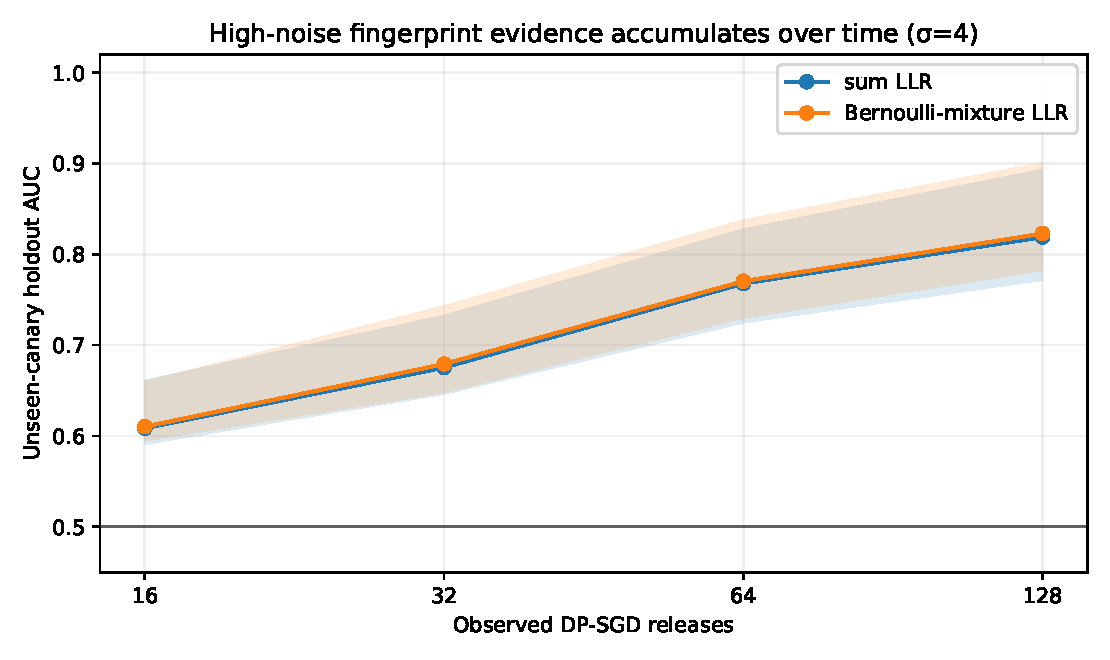
\includegraphics[width=\columnwidth]{figures/long_trajectory_auc.pdf}
  \caption{Unseen-canary AUC along nested prefixes of the same exact evolving DP-SGD trajectories at $\sigma=4$. Bands are 95\% paired identity-clustered bootstrap intervals.}
  \label{fig:long}
\end{figure}

Privacy exposure increases at the same time. Under the conservative replace-one zCDP calculation in Eq.~\ref{eq:zcdp}, the upper bound moves from $\epsilon=11.60$ at 16 releases to 17.57, 27.19, and 43.14 at 32, 64, and 128 releases. This comparison is not ``same privacy, longer observation''; each additional release spends privacy budget. The experiment demonstrates that an apparently weak short-window attack is not evidence that continued exposure is safe.

\subsection{Participation Rate Bounds the Accumulation Effect}

Figure~\ref{fig:q-sensitivity} and Table~\ref{tab:q-sensitivity} show that the strong trajectory result requires frequent participation. The 20-identity replication at $q=0.5$ gives AUC 0.805 at 128 releases, close to the original four-identity value 0.823 for the same mixture score. Reducing $q$ to 0.1 lowers AUC to 0.571; at $q=0.02$ it is 0.531, and at the ordinary-sampling proxy $q=0.004$ it is 0.503. The corresponding final-checkpoint AUCs are 0.730, 0.549, 0.517, and 0.498.

\begin{figure*}[t]
  \centering
  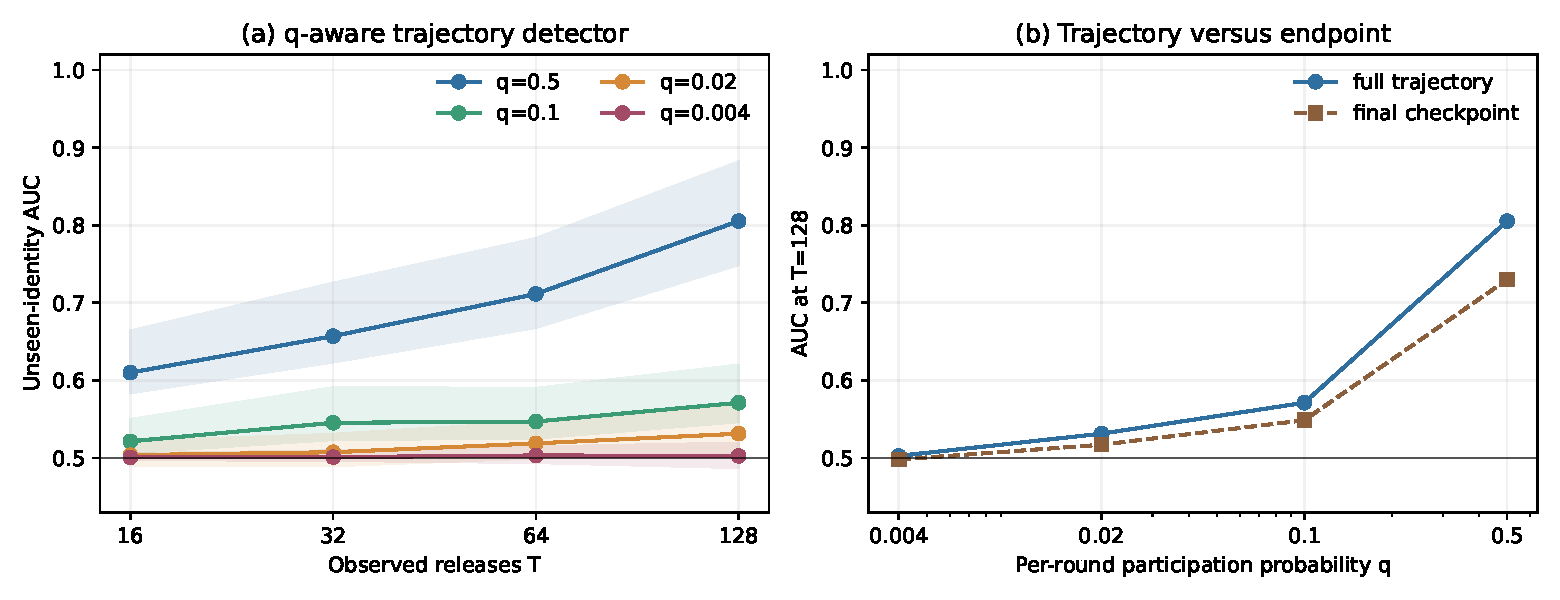
\includegraphics[width=.96\textwidth]{figures/q_sensitivity_endpoint.pdf}
  \caption{Participation-rate sensitivity at $\sigma=4$ on 20 unseen identities. (a) The $q$-aware trajectory score across nested prefixes; bands are 95\% identity/paired-sequence bootstrap intervals. (b) Full-trajectory and final-checkpoint candidate-loss AUC at 128 releases.}
  \label{fig:q-sensitivity}
\end{figure*}

\begin{table}[t]
\caption{Sensitivity and endpoint comparison at $T=128$. Intervals are identity/paired-sequence bootstrap intervals.}
\label{tab:q-sensitivity}
\centering
\resizebox{\columnwidth}{!}{%
\begin{tabular}{cccc}
\toprule
$q$ & $\E[\#\text{ inclusions}]$ & Trajectory AUC & Endpoint AUC \\
\midrule
0.5   & 64.0  & 0.805 $[0.749,0.882]$ & 0.730 $[0.686,0.801]$ \\
0.1   & 12.8  & 0.571 $[0.547,0.620]$ & 0.549 $[0.523,0.593]$ \\
0.02  & 2.56  & 0.531 $[0.503,0.568]$ & 0.517 $[0.494,0.551]$ \\
0.004 & 0.512 & 0.503 $[0.488,0.519]$ & 0.498 $[0.480,0.515]$ \\
\bottomrule
\end{tabular}
}
\end{table}

At $q=0.5,T=128$, the trajectory-minus-endpoint AUC gap is 0.076 with paired interval $[-0.001,0.148]$; this pilot therefore does not establish a statistically clear interface advantage. It does establish a participation boundary. At $q=0.004,T=128$, 61.7\% of positive runs realize zero inclusions, close to the theoretical $(1-q)^T=59.9\%$. Such runs are observationally identical to their negative pair. Repetition cannot accumulate a fingerprint that was usually never sampled, and the measured chance-level result prevents extrapolating the high-frequency canary finding to ordinary records over this horizon.

\subsection{Strong Final-Model Baselines Change the Interface Comparison}

Figure~\ref{fig:strong-endpoint} and Table~\ref{tab:strong-endpoint} compare attacks on the same paired runs for 80 new holdout identities. At the original learning rate, the final model has only 24.4\% accuracy on disjoint public query images after 128 updates. The $q=0.5$ trajectory AUC is 0.810, versus 0.693 for calibration-selected final-model LiRA and 0.667 for RMIA. The trajectory--strongest-endpoint gain is 0.117 with paired identity interval $[0.070,0.170]$. This establishes a gap in this low-utility condition, but it also warns against treating an impaired final model as the only endpoint baseline.

At the exploratory lower learning rate, accuracy reaches 66.2\%. The trajectory AUC remains 0.818, while LiRA rises to 0.830 and RMIA to 0.782. The trajectory-minus-best-endpoint difference is $-0.012$ with paired interval $[-0.043,0.020]$. Raw candidate-gradient alignment reaches 0.831 and differs from LiRA by only 0.001 $[-0.034,0.038]$. A calibration-selected linear fusion of LiRA and the $q$-aware trajectory assigns zero weight to the trajectory at $q=0.5,T=128$; fusing LiRA with raw alignment yields only 0.004 AUC gain $[-0.001,0.010]$. Thus this replication does not demonstrate a complementary membership signal beyond a strong final-model attack when the trained model is useful. At $q=0.1$, all attacks remain near 0.57--0.58 and no trajectory advantage is resolved. The differences across learning rates are exploratory comparisons of distinct training mechanisms, not a controlled fixed-utility causal effect.

\begin{figure*}[t]
  \centering
  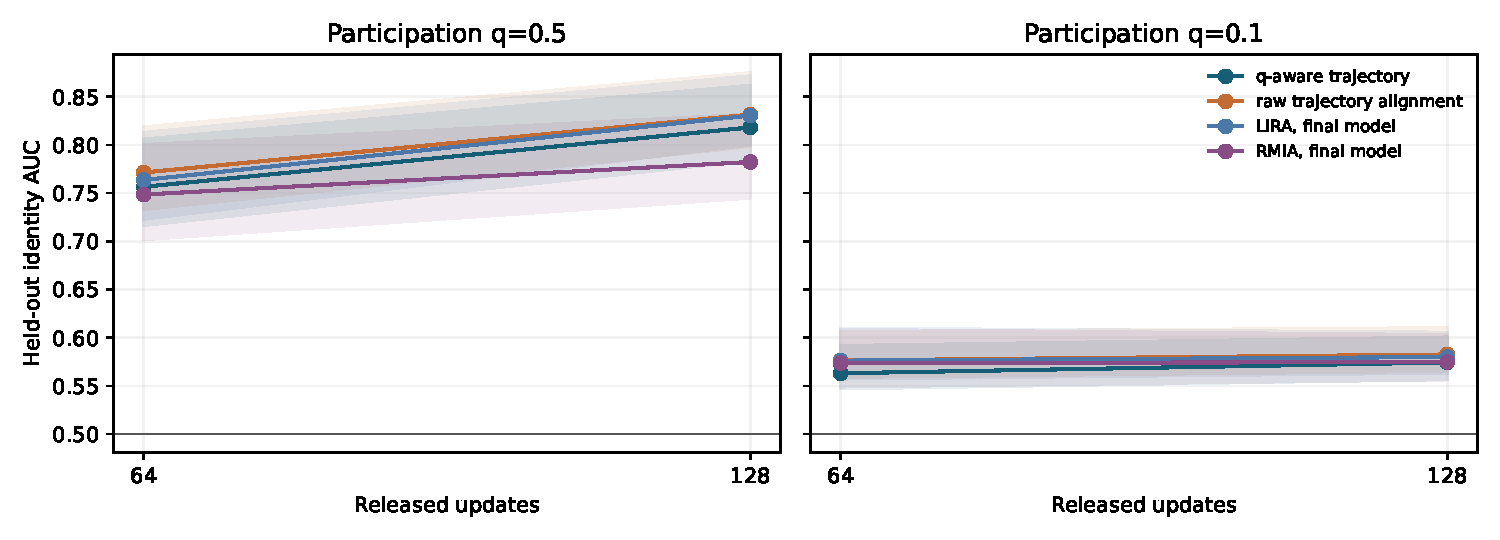
\includegraphics[width=.94\textwidth]{figures/trajectory_vs_endpoint_high_utility.pdf}
  \caption{Held-out AUC on 80 paired identities in the higher-utility setting ($\eta=0.005$, $\sigma=4$). Final-model LiRA and RMIA use 32 public OUT references; raw alignment and the q-aware likelihood use the entire trajectory. Bands resample identities.}
  \label{fig:strong-endpoint}
\end{figure*}

\begin{table*}[t]
\caption{Stronger final-model comparison at 128 releases, with 20 calibration and 80 evaluation identities per condition. The final column is the q-aware trajectory minus the strongest endpoint attack selected on calibration identities; intervals resample evaluation identities.}
\label{tab:strong-endpoint}
\centering
\resizebox{\textwidth}{!}{%
\begin{tabular}{cccccccc}
\toprule
$\eta$ & $q$ & Public accuracy & Trajectory & Raw alignment & LiRA & RMIA & Gain [95\% interval] \\
\midrule
0.05 & 0.5 & 0.244 & 0.810 & 0.784 & 0.693 & 0.667 & $+0.117\,[0.070,0.170]$ \\
0.05 & 0.1 & 0.243 & 0.563 & 0.562 & 0.537 & 0.531 & $+0.027\,[-0.002,0.057]$ \\
0.005 & 0.5 & 0.662 & 0.818 & 0.831 & 0.830 & 0.782 & $-0.012\,[-0.043,0.020]$ \\
0.005 & 0.1 & 0.663 & 0.574 & 0.583 & 0.580 & 0.575 & $-0.006\,[-0.022,0.011]$ \\
\bottomrule
\end{tabular}
}
\end{table*}

\subsection{Learned Sequence Models Do Not Outperform the Analytic Detector}

Table~\ref{tab:learned} compares the learned and analytic detectors on identical 16-round holdout trajectories. Conditional diffusion reaches AUC 0.944 at $\sigma=0.25$, only 0.015 above sum-LLR; the paired 95\% interval for the difference is $[-0.003,0.036]$. At $\sigma=1$ and $\sigma=4$, diffusion is worse by 0.032 and 0.043. The BiLSTM never materially improves on the analytic score.

\begin{table}[t]
\caption{Holdout AUC for analytic and learned 16-round detectors.}
\label{tab:learned}
\centering
\begin{tabular}{ccccc}
\toprule
$\sigma$ & Sum LLR & Mix. LLR & BiLSTM & Diffusion \\
\midrule
0.25 & 0.929 & 0.903 & 0.900 & 0.944 \\
1.00 & 0.884 & 0.857 & 0.864 & 0.852 \\
4.00 & 0.609 & 0.610 & 0.610 & 0.566 \\
\bottomrule
\end{tabular}
\end{table}

The learned models have two disadvantages in this regime. First, only four calibration identities are available, whereas the analytic score encodes the known Gaussian channel directly. Second, at high noise the conditional feature sequence contains little round-level information; a more expressive posterior model cannot recover information that is not present in its inputs. In this pilot comparison, the demonstrated improvement comes from longer exposure and a matched fingerprint rather than from a learned sequence model outperforming the analytic detector.

\subsection{Closed-Gallery Record Linkage and Distribution Confounds}

Accumulated evidence can identify a real record when it is present in an auxiliary gallery. Figure~\ref{fig:gallery} and Table~\ref{tab:gallery} report the larger matched-background replication at 128 releases and $\sigma=4$. Each distribution has 60 retrieval trials across 30 distinct target identities. Exact top-1 is 13.3--15.0\%, compared with 3.1\% at random, and top-5 is 36.7--48.3\%, compared with 15.6\% at random. This is weaker than the original ten-identity pilot's 15--30\% top-1 range, which illustrates why replication matters.

\begin{figure}[t]
  \centering
  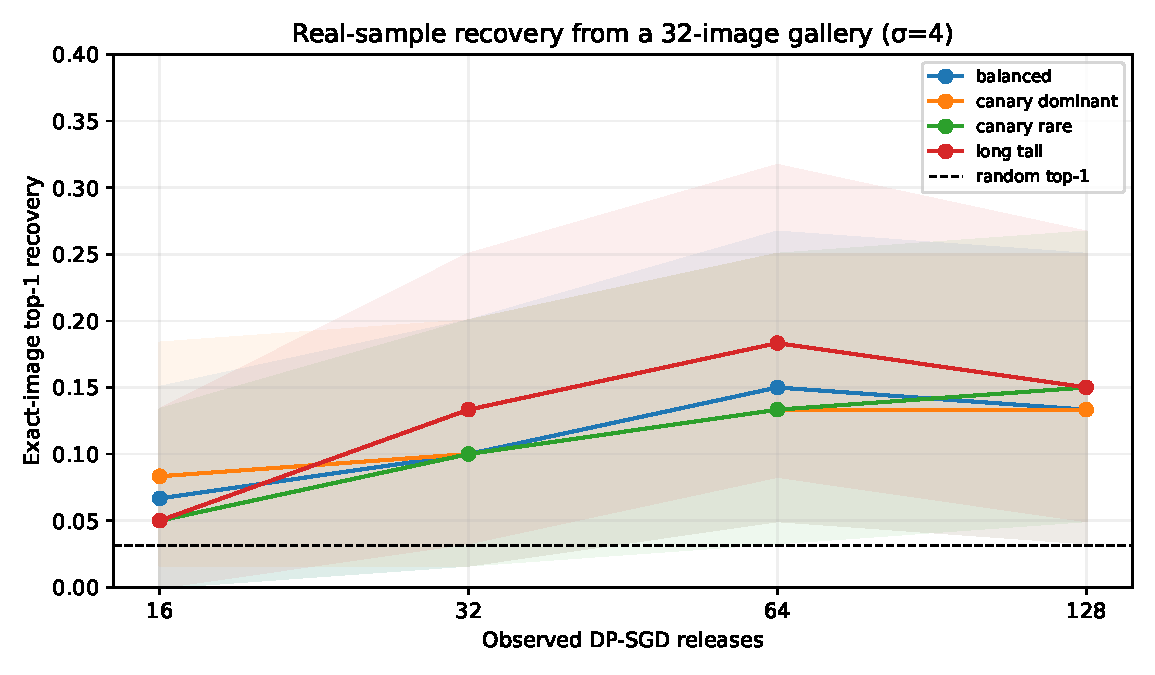
\includegraphics[width=\columnwidth]{figures/gallery_recovery_replication.pdf}
  \caption{Exact record recovery from a 32-image auxiliary gallery on 30 held-out target identities, two runs per identity and distribution. Bands resample identities.}
  \label{fig:gallery}
\end{figure}

\begin{table*}[t]
\caption{Closed-gallery recovery replicated on 30 identities per distribution with a matched public background at 128 releases ($\sigma=4$). Open-gallery metrics remove the true image before retrieval.}
\label{tab:gallery}
\centering
\begin{tabular}{lcccccc}
\toprule
Private distribution & Exact top-1 & Exact top-5 & Digit match & Same-class top-1 & Open digit & Open MSE \\
\midrule
Balanced & 0.133 & 0.433 & 0.167 & 0.650 & 0.100 & 0.146 \\
Long-tail & 0.150 & 0.483 & 0.183 & 0.600 & 0.117 & 0.150 \\
Canary class rare & 0.150 & 0.417 & 0.167 & 0.683 & 0.100 & 0.145 \\
Canary class dominant & 0.133 & 0.367 & 0.183 & 0.600 & 0.150 & 0.150 \\
\midrule
Random / class-only baseline & 0.031 & 0.156 & -- & 0.317 & 0.071 & 0.147 \\
\bottomrule
\end{tabular}
\end{table*}

Same-class top-1 is 0.60--0.68, above the 0.317 expected success of uniform guessing within the correct digit. Thus, matched-background rankings contain some image-specific evidence beyond digit recognition. Exact top-1 intervals remain broad, however; the balanced condition's identity-bootstrap interval is $[0.033,0.250]$. Recovery at 128 releases is also not uniformly better than at 64, so the figure does not support monotone exact reconstruction.

The mismatched-background control exposes a sharper failure mode. Using a balanced public background on canary-dominant private data yields 100\% digit agreement and 100\% open-gallery digit agreement, yet same-class top-1 is 25\%, below the 31.7\% label-only random baseline. The attack detects a population-level class shift, then guesses among images of that class. Conversely, mismatch reduces exact top-1 from 15.0\% to 6.7\% for both long-tail and rare-class data. A trajectory audit that reports only label match or top-$k$ can therefore mistake distribution leakage for record recovery.

When the true image is removed, matched-background digit agreement remains 10--15\% versus 7.1\% at random, indicating at most limited semantic leakage. The output is still another gallery image, and pixel MSE is close to the 0.149 random baseline. This control prevents us from interpreting gallery selection as generative reconstruction.

\section{Security Implications}

\subsection{Audit the Interface, Not Only the Final Model}

Standard composition-based DP-SGD accounting provides a valid privacy bound even when the sequence of intermediate updates is exposed. When only a final iterate is released, however, tighter hidden-state analyses may apply under additional assumptions because later noisy iterations can amplify the privacy of earlier contributions~\cite{feldman2018iteration,ye2022hidden}. Exposing intermediate states therefore does not invalidate standard composition; it changes the observable mechanism and can remove amplification available in a hidden-state analysis. Empirically, our stronger LiRA comparison finds no resolved trajectory advantage in the higher-utility setting; access to more observations alone is not evidence that this particular attack extracts more membership information. Systems should inventory gradient telemetry, intermediate checkpoint access, crash dumps, optimizer state, and federated-server visibility, then match both formal accounting and empirical auditing to the strongest interface actually exposed.

The fact that $\sigma=4$ sounds large does not imply strong end-to-end privacy. For fixed-size replacement and no amplification, our conservative bound reaches 43.14 after 128 releases. A production deployment should use an accountant matched to its sampler and adjacency, enforce a total budget, and stop releases when that budget is exhausted. Release minimization is a security control in its own right.

\subsection{Use Natural Canaries and Identity-Aware Controls}

Canaries provide known ground truth, but their design determines what an audit measures. An extreme outlier can exaggerate leakage; a weak canary can miss a bug. Our canaries are ordinary held-out MNIST records from the same data distribution and use the same clipping rule as population records. The sensitivity study shows that scheduling matters as much as canary content: the strong $q=0.5$ result attenuates at $q=0.1$ and disappears within 128 rounds at $q=0.004$. Audits should therefore match both the record distribution and the deployment's actual participation process.

For candidate recovery, class balance and background estimation are part of the threat model. We recommend at least four controls: a random gallery baseline, a same-class rank, removal of the true target, and a mismatched public background. Without them, semantic or distribution leakage can be reported as individual reconstruction.

\subsection{Analytic Baselines Before Learned Denoisers}

When the release noise is Gaussian and the candidate shift is computable, the matched LLR is the natural first baseline. A learned model should be compared against it on the same observations, identities, and model states. In our pilot, diffusion offers no high-noise advantage. Learned priors may matter when the fingerprint is only partially known, the background is structured, or the task is open-set generation, but those settings add assumptions that must be stated and controlled.

\section{Limitations and Future Work}

Our evidence is deliberately narrow. First, all exact trajectories use a small MNIST CNN and batch size eight. High-dimensional natural images, transformers, adaptive optimizers, augmentation, and larger batches may change fingerprint energy and background variance. The next evaluation should preregister hyperparameters and repeat the identity-holdout design on Fashion-MNIST, CIFAR-10, and a small language model.

Second, the strongest results use $q=0.5$, substantially above the approximately $B/N=0.004$ inclusion probability of an ordinary record. Our new sensitivity study measures the resulting boundary: AUC falls to 0.503 at $q=0.004,T=128$. This does not show that ordinary participation is always safe; it shows that the current horizon and detector provide no evidence of leakage in that condition. Longer runs, larger training populations, multiple epochs, and user-level participation require separate tests.

Third, the observer has full white-box model and gradient access and knows the candidate image and label. This matches an internal auditor or federated server, not a remote user. Partial-coordinate, quantized, secure-aggregation, stale checkpoint, and unknown-label variants are necessary to map the boundary of the attack. Our background estimator also uses public data representative of the private distribution; the mismatch experiment shows the cost of violating that assumption.

Fourth, the empirical units remain limited. The original holdout study has four identities and 48 positive/negative trajectories per condition. The sensitivity study improves identity coverage to 20 but has only three repetitions per identity and one model architecture. The strong-endpoint comparison has 80 unseen identities but only one paired run per identity and two learning rates; the higher-utility rate was selected in an exploratory calibration screen. Thirty-two OUT reference models provide only a finite approximation to LiRA and RMIA, and neither baseline is asserted to be optimal. The gallery replication includes 30 identities and two repetitions per distribution; its exact top-1 range corresponds to only 8--9 successful retrievals out of 60 trials per distribution. Cluster bootstrap intervals reflect independent identities but cannot replace replication on other architectures and datasets.

Fifth, AUC is not an empirical DP lower bound. Estimating $\epsilon$ requires valid confidence bounds on false-positive and false-negative events under a precisely specified neighboring-dataset experiment. Our study instead measures discrimination and retrieval for a natural-record distribution. It complements, rather than replaces, formal accounting and tight DP audits.

Finally, closed-gallery re-identification is not unknown-image reconstruction. A stronger next step is to exclude the target from every public bank, optimize a public generator's latent code against the cumulative trajectory likelihood, and lock the inversion procedure on public validation data before evaluating unseen targets. It should be scored against random, class-mean, same-class nearest-neighbor, prior-only, and clean-gradient controls. Until that gate is passed, ``record linkage'' is the correct description.

\section{Conclusion}

\method~demonstrates a bounded property of white-box DP-SGD exposure: a weak high-noise fingerprint can become informative when a record participates frequently and matched evidence is accumulated over the training trajectory. On exact evolving CNN runs at $\sigma=4$ and $q=0.5$, unseen-canary AUC reaches about 0.81 at 128 releases. The sensitivity study prevents a broader claim: AUC falls to 0.571 at $q=0.1$ and to chance at the ordinary-sampling proxy $q=0.004$. A larger paired study further shows why the endpoint comparator matters: trajectory AUC exceeds final-model LiRA in a low-utility training condition, but LiRA matches it when the model retains 66\% public-query accuracy, and their fusion provides no clear gain. More noise still improves privacy at fixed exposure, the learned diffusion baseline does not outperform the analytic detector, and distribution mismatch can create misleading class-level success. The practical conclusion is to match auditing to actual participation and interface access, use strong same-data baselines, and distinguish known-gallery identity leakage from semantic shortcuts and open reconstruction.

\section*{Ethical Considerations}

This work studies privacy attacks to improve auditing and system design. All experiments use MNIST and synthetic inclusion decisions; no human-subject or sensitive dataset is used. Releasing attack code could lower the cost of white-box record linkage, but the required access is already privileged and the method is a standard Gaussian likelihood test. We reduce misuse risk by stating the access assumptions, omitting claims of unknown-image reconstruction, and pairing the attack with concrete mitigations: correct composition, release minimization, access control, and identity-aware auditing. The artifact contains only public data instructions and aggregate results, not private user records.

\section*{Open Science}

An anonymized artifact accompanies the submission. It contains the complete PyTorch implementation, fixed configurations, tests for per-record gradients, clipping and update correctness, saved aggregate CSV results, and scripts that reproduce the paper figures. The MNIST CSV is not redistributed; the artifact documents its expected format and records its SHA-256 digest. The repository also includes negative and mismatch controls and does not overwrite completed runs. Row-level canary identifiers and large intermediate tensors are excluded from the review artifact; they can be regenerated from the public dataset and fixed seeds. The anonymous artifact link is supplied separately in HotCRP.

\section*{LLM usage considerations}

LLMs were used for editorial purposes in this manuscript, and all outputs were inspected by the authors to ensure accuracy and originality. An LLM also assisted with implementation scaffolding and consistency checks. It was not used to generate experimental observations: all reported values were computed by the saved code from fixed configurations and checked against exported CSV files. The human authors remain responsible for the method, literature review, claims, references, code, and results. No proprietary or sensitive dataset was sent to an LLM. Experiments used the smallest models sufficient to test the hypotheses, ran on CPU, and reused paired trajectories to reduce computation. The learned BiLSTM and diffusion models are scientific baselines in the method, not external LLM services.

\bibliographystyle{IEEEtran}
\bibliography{refs}

\appendices

\section{Implementation and Validation Details}

The implementation uses vectorized per-record automatic differentiation. A unit test compares vectorized gradients with a loop over individual records. Other tests verify global-norm clipping, the identity between the saved noisy release and actual parameter update, deterministic paired runs, disjoint split roles, likelihood calculations, candidate permutation equivariance, endpoint-prefix selection, and negative controls. A separate result check verifies that lower-$q$ inclusion schedules are subsets of their paired higher-$q$ schedules and that negative endpoint scores are identical across $q$ conditions.

For every trajectory round, candidate and public-background gradients are computed at the pre-update model state. The private batch is sampled next, its per-record gradients are clipped, and independent Gaussian noise is added to the sum. The stored observation is the averaged noisy gradient actually used in the update. No clean private gradient or sampled noise is passed to an attack.

The fixed-access experiment uses exact one-dimensional sufficient-statistic simulation rather than allocating full Gaussian vectors. This is algebraically equivalent for the matched detector and permits 20,000 observations per hypothesis, template, and noise level. Shared standard-normal draws pair the noise conditions.

\section{Additional Numerical Results}

\begin{table}[h]
\caption{Long-trajectory sum-LLR results and conservative privacy bounds.}
\centering
\begin{tabular}{ccccc}
\toprule
$T$ & AUC & Gain vs. 16 & 95\% interval & $\epsilon$ upper \\
\midrule
16 & 0.609 & 0.000 & $[0,0]$ & 11.60 \\
32 & 0.675 & 0.067 & $[0.010,0.124]$ & 17.57 \\
64 & 0.768 & 0.159 & $[0.094,0.218]$ & 27.19 \\
128 & 0.819 & 0.211 & $[0.144,0.272]$ & 43.14 \\
\bottomrule
\end{tabular}
\end{table}

In the original ten-identity gallery pilot, matched versus balanced-background exact top-1 at 128 releases is 0.20 versus 0.20 for balanced data, 0.25 versus 0.05 for long-tail data, 0.30 versus 0.15 for canary-rare data, and 0.15 versus 0.25 for canary-dominant data. The larger 30-identity replication in the main text gives lower matched top-1 rates and confirms the class shortcut: balanced-background canary-dominant retrieval has digit agreement 1.0 but same-class top-1 0.25.

\paragraph{Exploratory fixed-checkpoint controls.}
Separate fixed-checkpoint experiments provide an additional, exploratory check on learned denoising and inversion. Public-data Gaussian and neural priors reduce unseen-gradient squared error at moderate noise, but at $\sigma=4$ and 64 repeated releases their errors remain 0.353 and 0.345 versus 0.365 for the prior alone. Pixel inversion on nine images does not outperform a public class-mean image. Because these controls use a small image set and are not part of the main trajectory evaluation, we do not use them to support an unknown-image reconstruction claim.

\section{Claim Checklist}

\begin{itemize}
  \item The paper claims repeated-release fingerprint detection and closed-gallery re-identification under white-box access.
  \item It does not claim that increasing $\sigma$ at fixed composition reduces privacy, that DP is violated, or that unknown images are reconstructed.
  \item It does not extrapolate the frequent-participation result to ordinary sampling: the $q=0.004,T=128$ condition is reported at chance.
  \item Reported $\epsilon$ values are conservative analytical upper bounds, not empirical privacy estimates.
  \item Learned models are compared on identical observations and holdout identities; their negative results are retained.
  \item All central claims and limitations appear in the main body rather than relying on this appendix.
\end{itemize}

\end{document}
